\section{The Riemann-Roch theorem}
Equipped with sheaf cohomology, I will prove the Riemann-Roch theorem
using the methods we have learnt.
\begin{lnote}
  The rest of this article will be concerned with algebraic curves. Thus,
  $X$ will always denote an irreducible, non-singular, complete algebraic
  curve over an algebraically closed field $k$. Such curves can be embedded
  in the projective space, see \cite{serre}. This allows us to assume that
  the field of rational functions $k(X)$ consists of functions $f/g$, where
  $f$ and $g$ are homogeneous polynomials over $k$ with $\deg f=\deg g$.
\end{lnote}

\subsection{Divisors and differentials}
Before tackling the Riemann-Roch theorem, I will quickly review two
constructions that we will need in the last two sections of this paper:
\emph{divisors} and \emph{differentials}. I use \cite{gathmann}
and \cite{serre} as my sources.

Like a sheaf, a divisor is an object that associates additional data to
an algebraic variety. Unlike sheaves, divisors contain \textbf{discrete}
data. More specifically, a divisor $D$ on $X$ associates an integer to
each point of $X$ and only finitely many of these integers are non-zero.
Then, we can represent the divisor as a formal linear combination
\[
  D=\sum_{P\in X}n_{P}P,
\]
where the integer $n_{P}$ is the value associated to the point $P$.
Now, two divisors can be added component by component so that divisors on
$X$ form an abelian group $\Div X$. Given a divisor $D$, I write $D(P)$
for the value $n_{P}$ associated to the point $P\in X$.
\begin{figure}[H]
  \centering
  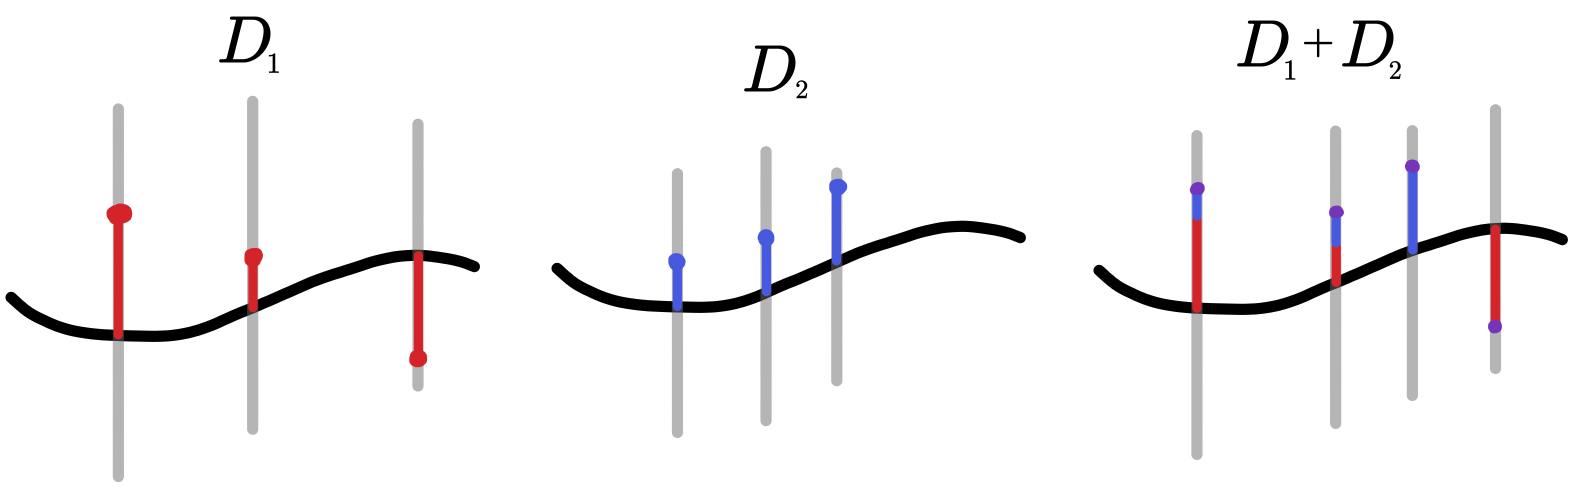
\includegraphics[width=\textwidth]{divisors}
  \caption{Visualising divisors and their sums.}
\end{figure}
I will now define the \emph{degree} of a divisor and an order relation on
the group of divisors. The degree of a divisor $D$ is simply the integer
\[
  \deg(D) = \sum_{P\in X} D(P).
\]
Next, I say $D$ is \emph{effective} and write $D\geq 0$ if $D(P)\geq 0$
for all $P\in X$. Then, given two divisors $D, D^{\prime}$, I can define
$D\geq D^{\prime}$ if the divisor $D-D^{\prime}$ is effective.

Important types of divisors are ones associated to a non-zero rational
function $f\in k(X)^{\times}$. For a point $P\in X$, the ring
$\mathscr{O}_{X,P}$ is a discrete valuation ring (DVR) with valuation
$\ord_{P}$. Then, the divisor of $f$ is defined as follows.
\[
  (f) = \sum_{P\in X}\ord_{P}(f)P.
\]
\begin{ex}
  Consider $X=\mathbb{P}^{1}$ and
  \[f(X_{0}, X_{1})=\frac{X_{1}-X_{0}}{X_{1}}\in k(\mathbb{P}^{1}).\]
  Since $f(X_{0}, X_{1})$ is a unit in the the local rings
  $\mathscr{O}_{X,P}$ for $P\neq [1:0], [1:1]$, we have $\ord_{P}(f)=0$
  at those points $P$. The points $[1:0]$ and $[1:1]$ are contained in the
  affine piece $\mathbb{A}_{0}^{1}=\Set{[X_{0},X_{1}]\in\mathbb{P}^{1}\mid
    X_{0}\neq 0}$. The dehomogenised version of $f$ on $\mathbb{A}_{0}^{1}$ is
  given by $f(x)=\frac{x-1}x$. One can immediately see that
  $\ord_{P_{0}}(f)=-1$ for $P_{0}=[1:0]$ and $\ord_{P_{1}}(f)=1$ for
  $P_{1}=[1:1]$. Therefore,
  \[(f)=P_{1}-P_{0}.\]
\end{ex}
\begin{rem}
  The divisor of a rational function should be thought of as counting the
  orders of zeros and poles of the function.
\end{rem}
It is useful to consider a non-constant element $f$ of $k(X)$ as a morphism
$f:X\to\mathbb{P}^{1}_{k}$, because then pre-composition by $f$ defines a
homomorphism of fields
\[
  k\left(\mathbb{P}^1_k\right)\to k\left(X\right):g\mapsto g\circ f.
\]
Since homomorphisms of fields are always injective, this map
defines the inclusion $k\left(\mathbb{P}^{1}_{k}\right)\subseteq k\left(X\right)$.
This fact can be used to define a homomorphism
$f^{\ast}:\Div\left(\mathbb{P}^{1}_{k}\right)\to\Div\left(X\right)$ in the
following way \cite{hartshorne}. Firstly, suppose $Q$ is a point of
$\mathbb{P}^{1}_{k}$ and let $t$ be a local uniformiser of
$\mathscr{O}_{\mathbb{P}^{1},Q}$. Then, $t$ can be seen as a function in $k(X)$
and one can define
\[
  f^{\ast}(Q)=\sum_{f(P)=Q}\ord_{P}(t)\,P.
\]
This definition is independent of the choice of local uniformiser: Suppose
$t^{\prime}$ is another local uniformiser of $\mathscr{O}_{\mathbb{P}^{1},Q}$.
Then, there is a unit $u$ of $\mathscr{O}_{\mathbb{P}^1,Q}$ such that $t^{\prime}=ut$. 
Since $u$ is a unit, its denominator and numerator do not vanish at $Q$. Thus, 
the denominator and the numerator of the corresponding function $u\circ f$ in $k(X)$ 
do not vanish at $P$, as $f(P)=Q$. Therefore, $u\circ f$ is a unit of
$\mathscr{O}_{X,P}$, and so, $\ord_{P}(t)=\ord_{P}(t^{\prime})$. Furthermore, this
definition can be linearly extended for an arbitrary divisor
$D\in\Div(\mathbb{P}^{1}_{k})$. Now, the following lemma will be useful.
\begin{lemm}\label{lemm:deg_of_induced}
  If $f\in k(X)\setminus k$, then for the induced morphism $f^{\ast}:\Div\left(
    \mathbb{P}^{1}_{k}\right)\to\Div\left(X\right)$ we have
  \[
    \deg\left(f^{\ast}(D)\right)=[k(X):k(\mathbb{P}^{1}_{k})]\,\deg(D).
  \]
\end{lemm}
\begin{proof} % TODO: Give a proof sketch
  See Proposition 6.9 of \cite{hartshorne} chapter II.
\end{proof}
\begin{cor}\label{cor:rational_deg_zero}
  Suppose $f\in k(X)^{\times}$. Then, $\deg\left((f)\right)=0$.
\end{cor}
\begin{proof}
  If $f$ is a constant, then the statement is immediate. Thus, assume
  $f$ is not a constant. Then, one can write
  $(f)=f^{\ast}(0)-f^{\ast}(\infty)$ and compute the degree:
  \[
    \deg\left((f)\right)=\deg(f^{\ast}(0))-\deg(f^{\ast}(\infty))
    =[k(X):k(\mathbb{P}^{1}_{k})]-[k(X):k(\mathbb{P}^{1}_{k})]=0.
  \]
\end{proof}
\begin{rem}
  Note that divisors of rational functions form a group since
  $(f)+(g)=(fg)$. Then, we can take the quotient of $\Div X$ by this group.
  The quotient is called the Picard group $\Pic X$ and its elements are
  called \textbf{divisor classes}. Thus, there is an equivalence relation on
  $\Div X$ such that
  \[
    D\sim D^{\prime}\iff \exists f\in k(X)^{\times},\ D^{\prime}=D+(f).
  \]
  Then, $D$ and $D^{\prime}$ are said to be \textbf{linearly equivalent}.
\end{rem}

In this paper, I will use divisors to control the ``order of vanishing'' of 
a rational function $f\in k(X)^{\times}$. For example, if I want to allow 
$f$ to have a pole only at some point $P\in X$ with order at most $2$,
I can express this requirement in the following way. Define a divisor
$D=-2P$ and require that $(f)\geq D$. Conventionally, we would actually
set $D=2P$ and require that $(f)\geq -D$. This leads us to define the
sheaf $\mathscr{O}_X(D)$ of such functions:
\[
  \left(\mathscr{O}_X(D)\right)(U)=\Set{f\in k(X)\mid
  \forall P\in U,\ \ord_{P}(f)\geq -D(P)}
\]
\begin{figure}[H]
  \centering
  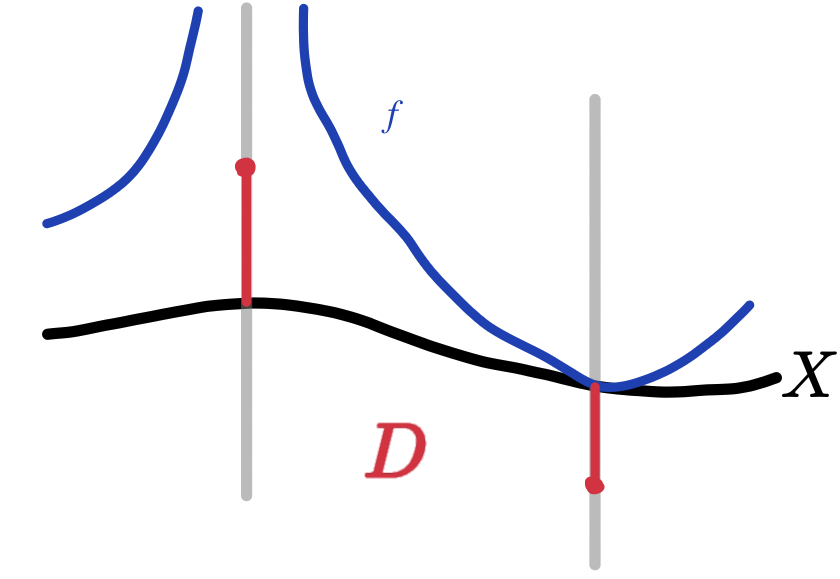
\includegraphics[width=.6\textwidth]{divisor_section}
  \caption{A section of the sheaf $\mathscr{O}_X(D)$.}
\end{figure}
\begin{prop}
  The sheaves $\mathscr{O}_X(D)$ are quasi-coherent for every divisor $D$.
\end{prop}
\begin{proof}
  Firstly, $\mathscr{O}_X(D)$ is clearly a sheaf of $\mathscr{O}_{X}$-modules:
  If $f, g\in\mathscr{O}_X(D)(U)$, then it is clear that
  \[
    \forall P\in U,\ \ord_{P}(f+g)\geq -D(P).
  \]
  Moreover, if $h\in\mathscr{O}_{X}(U)$, then multiplying $f$ by $h$ only
  increases the order at all points, since $\ord_{P}(h)$ is never negative
  on $U$.

  Now, suppose $U\subseteq X$ is an affine open set and let $P\in U$ be a
  point where $D$ is non-zero. Then, take the open set
  $U_{P}^{\prime}\subseteq U$, which doesn't contain any of the other points
  where $D$ is non-zero. One can find a function $\phi_{P}\in k(X)$ in some
  neighbourhood $U_{P}\subseteq U_{P}^{\prime}$ of $P$ such that $(\phi_{P})=P$
  (by \cite[Lemma 7.5.6]{gathmann}). Now, multiplication by $\phi_{P}$
  defines an isomorphism $\mathscr{O}_X(D)(U_{P})\to \mathscr{O}_{U_{P}}$.
  Since quasi-coherence can be checked locally, this finishes the proof.
  % TODO: Can we not just set phi_P to be the local uniformizer of O_{X,P}?
\end{proof}
The following proposition will also be useful later.
\begin{prop}\label{prop:global_sec_negative_divisor}
  If a divisor $D$ has negative degree, then $H^{0}(X,\mathscr{O}_X(D))=0$.
\end{prop}
\begin{proof}
  Suppose $f\in H^{0}(X,\mathscr{O}_X(D))$. Then, $(f)\geq -D$
  so that $\deg((f))\geq -\deg(D)$, but this implies $\deg(D)\geq 0$
  by Prop.~\ref{cor:rational_deg_zero}, which contradicts the assumption on
  $D$.
\end{proof}

I will now turn to discussing differentials. In geometry, spaces are often
studied locally by looking at their tangent spaces. But the notion of
the tangent space does not translate directly to algebraic geometry,
and we would like to have a more algebraic alternative. It turns out that it
is easier to give an algebraic definition of the \emph{cotangent space},
the dual space of the tangent space. The cotangent space can be defined
abstractly as a module of differentials, which makes it nice to work with from
an algebraic perspective. I will not attempt to make the connection to
geometry more apparent since giving geometric motivation for the definitions
would take us too far from the focus of the article, and thus I leave it out.
For a soft exposition of differential forms in analysis, I recommend reading
Terence Tao's excellent article \cite{tao}.
\begin{defin}
  For a commutative algebra $F$ over a field $k$, the module of
  $k$-differentials of $F$ is the free $F$-module $\Omega(F)$ generated
  by the symbols $df$ for $f\in F$ with the following rules.
  \begin{itemize}
    \item $d(f+g)=df+dg$ for $f, g\in F$,
    \item $d(fg)=f\,dg+g\,df$ for $f, g\in F$,
    \item $da = 0$ for $a\in k$.
  \end{itemize}
\end{defin}
Note that this definition implies that the differential map $d:F\to\Omega(F)$
is $k$-linear, as $d(af)=a\,df+f\,da=a\,df$ for $a\in k$. I will write
$\Omega$ for the module $\Omega\left(k(X)\right)$.
\begin{prop}
  Suppose $t$ is a local uniformiser of $\mathscr{O}_{X,P}$ at some
  point $P\in X$. Then, $\Omega$ is spanned by the differential $dt$.
\end{prop}
\begin{proof}
  First, consider the $k$-vector space
  $\Omega\left(\mathscr{O}_{X,P}\right)/\mathfrak{m}_{P}\Omega\left(
    \mathscr{O}_{X,P}\right)$, where
  $\mathfrak{m}_{P}$ is the maximal ideal of $\mathscr{O}_{X,P}$. I will show
  that this space is spanned by the differential $dt$ and then apply
  Nakayama's lemma. Thus, take an element $\sum f_{i}\,dg_{i}\in\Omega\left(
    \mathscr{O}_{X,P}\right)$. As $\mathscr{O}_{X,P}/\mathfrak{m}_{P}=k$,
  one can write
  \[
    f_{i}=m_{i}+a_{i}\text{ and }g_{i}=m_{i}^{\prime}+a_{i}^{\prime}
    \text{, where } m_{i}, m_{i}^{\prime}\in\mathfrak{m}_{P}
    \text{ and } a_{i}, a_{i}^{\prime}\in k.
  \]
  Then, $f_{i}\,dg_{i}\equiv a_{i}\,dg_{i}$ modulo
  $\mathfrak{m}_{P}\Omega\left(\mathscr{O}_{X,P}\right)$.
  Furthermore, since $\mathfrak{m}_{P}=(t)$, there is
  $r_{i}\in\mathscr{O}_{X,P}$ such that $m_{i}^{\prime}=r_{i}t$. One can again
  write $r_{i}=m_{i}^{\prime\prime}+a_{i}^{\prime\prime}$ so that
  $m_{i}^{\prime}=a_{i}^{\prime\prime}t+m_{i}^{\prime\prime}t$. Therefore,
  \[
    dg_{i}=d\left(m_{i}^{\prime}+a_{i}^{\prime}\right)=dm_{i}^{\prime}
    =a_{i}^{\prime\prime}\,dt+m_{i}^{\prime\prime}\,dt+t\,dm_{i}^{\prime\prime}
    \equiv a_{i}^{\prime\prime}\,dt.
  \]
  and thus
  \[
    \sum f_{i}\,dg_{i}\equiv \sum a_{i}a_{i}^{\prime\prime}\,dt.
  \]
  Since I have shown that $dt$ forms a basis of
  $\Omega\left(\mathscr{O}_{X,P}\right)/\mathfrak{m}_{P}\Omega\left(
    \mathscr{O}_{X,P}\right)$, I can apply Nakayama's lemma
  (see \cite[Proposition 2.8]{am}), which implies that $dt$ also generates
  $\Omega\left(\mathscr{O}_{X,P}\right)$ as an $\mathscr{O}_{X,P}$-module.
  Now, suppose $f\in k(X)$. Such a function has an expansion
  \[
    f=a_{-n}t^{-n}+a_{-n+1}t^{-n+1}+\cdots +a_{-1}t^{-1}+ut^{n},
  \]
  where $a_{i}\in k$, $u$ is a unit in $\mathscr{O}_{X,P}$ and $n\geq 0$.
  Then,
  \[
    df=-na_{-n}t^{-n-1}\,dt+\cdots-a_{-1}t^{-2}\,dt+d\left(ut^{n}\right)
  \]
  Since $ut^{n}\in\mathscr{O}_{X,P}$, the differential $df$ is in the span
  of $dt$. It is easy to see that the statement follows from here.
\end{proof}
This proposition lets us to define the order of a differential
$\omega\in\Omega$ as follows. Write $\omega=f\,dt$ for $f\in k(X)$. Then,
\[
  \ord_{P}(\omega)=\ord_{P}(f).
\]
Now, one can define the divisor $(\omega)$ of $\omega$ in the same way as
the divisor of a rational function:
\[
  (\omega)=\sum_{P\in X}\ord_{P}(\omega)P.
\]
It turns out that divisors of this kind are all linearly equivalent: suppose
$\omega_{1}=f_{1}\,dt$ and $\omega_{2}=f_{2}\,dt$. Then,
\[
  \omega_{1}=\frac{f_{1}}{f_{2}}\, f_{2}\,dt=\frac{f_{1}}{f_{2}}\omega_{2}
  \implies (\omega_{1})=\left(\frac{f_{1}}{f_{2}}\right)+(\omega_{2}).
\]
Thus, the divisors of differentials lie in the same divisor class called the
\emph{canonical class}. A representative of the class is called the
\emph{canonical divisor} $K_{X}$.

Next I define a module of differentials related to a divisor $D$
on $X$ in the same way as we defined the sheaf $\mathscr{O}_X(D)$:
\[
  \Omega(D)=\Set{\omega\in\Omega\mid \forall P\in X,\ \ord_{P}(\omega)
  \geq D(P)}.
\]
(in the modern literature one requires $\ord_{P}(\omega)\geq -D(P)$
to match the definition of $\mathscr{O}_X(D)$, but here I follow \cite{serre}
with the notation). Lastly, I will define the \emph{residue} of a
differential, which will be the main ingredient in the proof of Serre
Duality in the next section.
\begin{defin}
  Let $\omega=f\,dt\in\Omega$, where $t$ is a local uniformiser of
  $\mathscr{O}_{X,P}$ for some point $P\in X$. Then, $f$ can be embedded
  in the ring $k((t))$ of formal series over $k$, where it has a series
  expansion in terms of $t$:
  \[
    f=\sum_{i\geq n}a_{i}t^{i},
  \]
  where $n\in\mathbb{Z}$ and $a_{i}\in k$. Then, the residue of $\omega$
  at $P$ is defined as $\res_{P}(\omega)=a_{-1}$.
\end{defin}
\begin{lnote}
  After this point, it is easy to get lost in all the preliminary
  results we need to prove about residues. It is not forbidden to skip
  to Subsection~\ref{ss:riemann_roch_proof} if this happens.
\end{lnote}
A priori, this definition depends on the local uniformiser $t$, and thus
I need to show that the definition is indeed independent of the choice
of a local uniformiser. I will only give a proof sketch, but for a more
detailed proof, see \cite{serre}.
\begin{lemm}\label{lemm:res_quotient}
  For a non-zero function $f$, we have $\res_{P}(df/f)=\ord_{P}(f)$.
\end{lemm}
\begin{proof}
  If $t$ is a local uniformiser of $\mathscr{O}_{X,P}$, then $f$ can be
  written as $f=ut^{n}$, where $n=\ord_{P}(f)$. Then,
  \[
    df/f = \frac{t^{n}\,du + nut^{n-1}\,dt}{ut^{n}}=du/u+n\,dt/t.
  \]
  Thus, $\res_{P}(df/f)=\res_{t}(du/u)+n$, but since $u$ is a unit in
  $\mathscr{O}_{X,P}$, the residue $\res_{t}(du/u)$ is clearly zero.
\end{proof}
\begin{prop} % TODO: Check differential stuff after this point
  Fix a point $P\in X$ and let $t$ and $u$ be two local uniformisers of
  $\mathscr{O}_{X,P}$. Denote by $\res_{t}$ and $\res_{u}$ the function
  $\res_{P}$ calculated using $t$ and $r$ respectively. Then,
  $\res_{t}(\omega)=\res_{u}(\omega)$ for all differentials $\omega\in\Omega$.
\end{prop}
\begin{proof}[Proof sketch]
  Suppose $f\in k(X)$ is a rational function with a series expansion
  \[
    f=\sum_{i\geq n}a_{i}u^{i},
  \]
  in $u$. Then, it is possible to construct a module of differentials, where
  \[
    df=\left(\sum_{i\geq n}ia_{i}u^{i-1}\right)\,du.
  \]
  This is probably the most non-trivial statement of the proof, and the
  construction is laid out by Serre \cite{serre}. Now, we can write a
  differential $\omega$ in this module as
  \[
    \omega = \sum_{n\geq 0}a_{n}\,du/u^{n}+\omega_{0},
  \]
  where $\omega_{0}$ is a differential with $\ord_{P}(\omega_{0})\geq 0$.
  Then, $\res_{u}(\omega)=a_{1}$ and $\res_{t}(\omega)=
  \sum a_{n}\res_{t}(du/u^{n})$. Now, concentrate first on the term
  $a_{1}\res_{t}(du/u)$. I can apply Lemma~\ref{lemm:res_quotient}
  to get $\res_{t}(du/u)=\ord_{P}(u)=1$. Therefore,
  \[
    \res_{t}(\omega) = a_{1}+\sum_{n>0}\res_{t}(du/u^{n}).
  \]
  Hence, it is enough to show that $\res_{t}(du/u^{n})=0$ for $n>0$.

  In characteristic zero, we can write
  \[
    du/u^{n}=d\left(-\frac1{(n-1)u^{n-1}}\right).
  \]
  But this immediately implies that $\res_{t}(du/u^{n})=0$ since
  differentiating a series can never result in a term of the form
  $a_{-1}t^{-1}$. The proof for positive characteristic follows from the
  statement in zero characteristic by an argument by Serre \cite{serre}.
\end{proof}
Now, I will prove the \emph{residue formula}, which is used in the proof
of Serre Duality.
\begin{thm}[Residue Formula]\label{thm:residue_theorem}
  For every differential $\omega\in\Omega$, we have that
  \[
    \sum_{P\in X}\res_{P}(\omega)=0.
  \]
\end{thm}
First I prove the theorem for the case when $X=\mathbb{P}^{1}_{k}$.
\begin{lemm}
  The residue formula holds for $X=\mathbb{P}^{1}_{k}$.
\end{lemm}
\begin{proof}
  Fix a differential $\omega=f\,dt$ on $X$. For convenience, I work with
  dehomogenised representation, and take $f$ to be a rational function
  in one variable $t$. This function has a partial fractions decomposition,
  which is a linear combination of terms of the form listed below. I will
  consider each type separately.
  \begin{description}[style=nextline]
    \item[Term of type $\omega=t^{n}\,dt$:] There are no poles at finite
          points, so the only pole could be at infinity. Changing to
          $u=1/t$, we have $dt=-u^{-2}\,du$ and
          \[\omega=(u^{-n})(-u^{-2}\,du)=\frac{du}{u^{n+2}}.\]
          Then, the residue clearly vanishes: $\res_{\infty}(\omega)=0$.
    \item[Term of type $\omega=\frac{dt}{t-a}$:] Clearly $\res_{a}(\omega)=1$,
          and there are no other poles at finite points. But there is also a
          pole at infinity. Again, changing to $u=1/t$, we get
          \begin{align*}
            f(u)&=\left(\frac{u}{1-au}\right)(-u^{-2}\,du)
            =-\frac1{u}\cdot\frac1{1-au}\,du \\
            &=-\frac1{u}\left(1+au+(au)^{2}+\cdots\right)\,du.
          \end{align*}
          Therefore, $\res_{a}(\omega)=-1$ and the residues of the two points
          cancel.
    \item[Term of type $\omega=\frac{dt}{(t-a)^{n}}$ for $n>1$:] Following
          a similar argument as above, one can check that in this case
          the residue is zero also at $a$ and $\infty$.
  \end{description}
\end{proof}
Let $X$ be a curve as before. Again, a non-constant function $\phi\in k(X)$
induces an embedding $k(\mathbb{P}^{1}_{k})\hookrightarrow k(X)$, and I hope
to use this embedding to apply the above lemma in the case of an arbitrary
curve $X$. Now, one can consider the trace map $\tr_{k(X)/k(\mathbb{P}^{1}_{k})}$
defined as follows \cite{milne}. Multiplication by an element
$\alpha\in k(X)$ defines a $k(\mathbb{P}^{1}_{k})$-linear map
$\alpha^{\ast}: E\to E: x\mapsto \alpha x$. Then, we simply define
$\tr_{k(X)/k(\mathbb{P}^{1}_{k})}(\alpha)$ to be the usual trace of this linear
transformation $\alpha^{\ast}$. Next I translate this definition to
differentials on $k(X)$. We can write any differential
$\omega\in\Omega(k(X))$ as $\omega=f\,d\phi$. Then, one can make the
following definition.
\[
  \tr:\Omega(k(X))\to \Omega(k(\mathbb{P}^{1}_{k}))
  :f\,d\phi\mapsto \left(\tr_{k(X)/k(\mathbb{P}^{1}_{k})}(f)\right)\,d\phi
\]
Finally, the residue formula is implied by the following lemma
\cite{serre}.
\begin{lemm}
  For every point $P\in\mathbb{P}^{1}_{k}$, we have
  \[
    \sum_{Q\in\phi^{-1}(P)}\res_{Q}(\omega)=\res_{P}(\tr(\omega)).
  \]
\end{lemm}

This finishes the subsection on divisors and differentials, and we 
are now ready to move on to discussing the Riemann-Roch theorem 
and Serre Duality.

\subsection{Proof of Riemann-Roch}\label{ss:riemann_roch_proof}
I am now able to state and prove an ``incomplete'' version of the
Riemann-Roch theorem, which I will make complete after proving Serre
Duality.

\begin{thm}[Riemann-Roch, cohomology version]
  \label{thm:riemann_roch_cohomology}
  For every divisor $D$ on $X$,
  \[
    h^{0}(X, \mathscr{O}_X(D))-h^{1}(X, \mathscr{O}_X(D))=\deg(D)+1-g,
  \]
  where $g=h^{1}(X, \mathscr{O}_{X})$ and $h^i(X,\mathscr{F})$
  denotes $\textnormal{dim}\left(H^i(X,\mathscr{F})\right)$.
\end{thm}
\begin{proof}
  One can use an induction argument, because any divisor $D$ can be
  obtained from the zero divisor by adding and subtracting points.
  Thus, I proceed by first proving the base case and then proving
  the induction step.

  \begin{description}[style=nextline]
    \item[base case$\big)$]
          Since $\mathscr{O}_X(0)=\mathscr{O}_{X}$ and $\deg(0)=0$,
          I need to verify that
          \[h^{0}(X, \mathscr{O}_{X})-h^{1}(X, \mathscr{O}_{X})=1-g.\]
          But note that the only globally defined regular functions
          on $X$ are constant and thus they form a one-dimensional vector
          space. Moreover, $h^{1}(X, \mathscr{O}_{X})=g$ by definition
          so that the equality holds.
    \item[induction step$\big)$]
          In the induction step I want to relate the 0th and the 1st
          cohomology groups of $\mathscr{O}_X(D)$ to the 0th and
          1st cohomology groups of $\mathscr{O}_X(D+P)$, where
          $P$ is some point. To do this, first note that
          $\mathscr{O}_X(D)$ is a subsheaf of $\mathscr{O}_X(D+P)$, since
          the orders of the sections of $\mathscr{O}_X(D+P)$ at $P$ are
          allowed to be smaller than the orders of the sections of
          $\mathscr{O}_X(D)$ at $P$. Thus, there is an exact sequence
          \[
          \begin{tikzcd}
            0\arrow{r} & \mathscr{O}_X(D)\arrow{r} & \mathscr{O}_X(D+P)\arrow{r}
            & Q\arrow{r} & 0,
          \end{tikzcd}
          \]
          where $Q$ is the quotient sheaf. The stalks of $Q$ are clearly
          zero away from $P$. The stalk at $P$ consists of zero and
          elements of the form $u/t^{n+1}$, where $t$ is the local
          uniformiser of $\mathscr{O}_{X,P}$, $u$ is a unit in
          $\mathcal{O}_{X,P}$, and $n$ is the order of $P$ in $D$.
          As $\mathcal{O}_{X,P}/(t)=k$, we can write $u=vt+r$,
          where $v\in\mathcal{O}_{X,P}$ and $r\in k$.
          Then,
          \[\frac{u}{t^{n+1}}=\frac{v}{t^n}+\frac{r}{t^{n+1}}.\]
          Since $v/t^n$ is an element of $\mathscr{O}_X(D)_{P}$, we conclude
          that every element of $\mathscr{O}_X(D+P)_{P}$ is equivalent to
          an element $r/t^{n+1}$ modulo $\mathscr{O}_X(D)_{P}$ for some
          $r\in k$. Therefore, $Q_{P}\cong k$ and $Q$ is the skyscraper sheaf
          $k_{P}$.

          Now we apply our cohomology machinery on the SES
          \[
          \begin{tikzcd}
            0\arrow{r} & \mathscr{O}_X(D)\arrow{r} & \mathscr{O}_X(D+P)\arrow{r}
            & k_{P}\arrow{r} & 0
          \end{tikzcd}
          \]
          to get the following exact sequence (using
          Prop.~\ref{prop:sky_cohom}).
          \[
          \begin{tikzcd}
            0\arrow{r} & H^{0}(X, \mathscr{O}_X(D))\arrow{r}
            & H^{0}(X, \mathscr{O}_X(D+P))\arrow{r}
            & H^{0}(X, k_{P}) \\
            \arrow{r} & H^{1}(X, \mathscr{O}_X(D))\arrow{r}
            & H^{1}(X, \mathscr{O}_X(D+P))\arrow{r} & 0.
          \end{tikzcd}
          \]
          Now, this exact sequence of vector spaces implies the following
          equality.
          \[
          h^{0}(X,\mathscr{O}_X(D))-h^{0}(X, \mathscr{O}_X(D+P))
          +1-h^{1}(X,\mathscr{O}_X(D))+h^{1}(X,\mathscr{O}_X(D+P)) = 0.
          \]
          Therefore,
          \begin{align*}
            h^{0}(X,\mathscr{O}_X(D+P))&-h^{1}(X,\mathscr{O}_X(D+P)) \\
            =&\left(h^{0}(X,\mathscr{O}_X(D))-h^{1}(X,\mathscr{O}_X(D+P))\right)
              +1 \\
            =&\deg(D)+1-g+1\quad\text{(by induction hypothesis)} \\
            =&\deg(D+P)+1-g.
          \end{align*}
          This is exactly the induction step we wanted to prove.
          We also need to prove
          \[
            h^{0}(X,\mathscr{O}_X(D-P))-h^{1}(X,\mathscr{O}_X(D-P))
            =\deg(D-P)+1-g,
          \]
          but we can run the same argument starting with the SES
          \[
          \begin{tikzcd}
            0\arrow{r} & \mathscr{O}_X(D-P)\arrow{r} & \mathscr{O}_X(D)\arrow{r}
            & k_{P}\arrow{r} & 0.
          \end{tikzcd}
          \]
  \end{description}
\end{proof}
\begin{lwarn}
  One would need to also prove that the cohomology groups are finite
  dimensional to begin with. See \cite{serre} for the details.
\end{lwarn}

This form of the theorem is not the most useful one for applications,
because computing $h^{1}(X,\mathscr{O}_X(D))$ is not easy. However, one can
get a nice expression for this space using the Serre Duality, which
I will prove in the next section:
\newtheorem*{thm:serre}{Theorem~\ref{thm:serre}}
\begin{thm:serre}[Serre Duality]
  If $X$ is an algebraic curve as before
  and $D$ is a divisor on $X$, there is an isomorphism
  \[
    \dual{D}\cong \diffs{D}.
  \]
  of $k$-vector spaces.
\end{thm:serre}
Since we are only interested in the dimension of $h^{1}(X,\mathscr{O}_X(D))$,
I will use the following lemma to give the dimension in terms of the
canonical divisor.
\begin{lemm}\label{lemm:diffs_dim}
  We have the following equality in dimensions.
  \[\dim\left(\Omega(D)\right)=h^{0}(X,\mathscr{O}_X(K_{X}-D))\]
\end{lemm}
\begin{proof}
  Write $K_{X}=(\omega_{0})$ with $\omega_{0}=f_{0}\,dt$ and fix a
  differential $\omega=f\,dt$. Then, $\omega=\frac{f}{f_{0}}\omega_{0}$
  and we have
  \[
    \omega\in\Omega(D)\iff (\omega)\geq D
    \iff\left(\frac{f}{f_{0}}\right)+(\omega_{0})\geq D\iff
    \frac{f}{f_{0}}\in H^{0}(X,\mathscr{O}_X(K_{X}-D)).
  \]
  In other words, the elements of $H^{0}(X,\mathscr{O}_X(K_{X}-D))$ are in
  bijection with the elements of $\Omega(D)\cong\dual{D}$.
\end{proof}
Now, this equality lets us write the ``complete'' form of the Riemann-Roch
theorem.
\begin{thm}[Riemann-Roch]\label{thm:riemann_roch}
  For every divisor $D$,
  \[
    h^{0}(X, \mathscr{O}_X(D))-h^{0}(X, \mathscr{O}_X(K_{X}-D))=\deg(D)+1-g,
  \]
  where $g=h^{1}(X, \mathscr{O}_{X})$.
\end{thm}

\subsection{An application to the classification of curves}
Before proving Serre Duality, I want to take some time to
look at an application of the Riemann-Roch theorem using \cite{hartshorne}
as my source. A major project in algebraic geometry is to give a
classification of different algebraic varieties. The Riemann-Roch theorem
helps us prove statements about curves based solely on topological data,
namely the genus of the curve. First, I give a formula for the degree
of the canonical divisor on a curve.
\begin{lemm}
  The degree of the canonical divisor $K_{X}$ is $2g-2$, where $g$ is the
  genus of $X$.
\end{lemm}
\begin{proof}
  Set $D=K_{X}$ so that the Riemann-Roch theorem yields
  \begin{align*}
    h^{0}(X,\mathscr{O}_X(K_{X}))-h^{0}(X,\mathscr{O}_{X})&=\deg(D)+1-g \\
    h^{1}(X,\mathscr{O}_{X})-1&=\deg(D)+1-g \\
    2g-2&=\deg(D),
  \end{align*}
  where $h^{0}(X,\mathscr{O}_X(K_{X}))=h^{1}(X,\mathscr{O}_{X})$ is given
  by Serre Duality.
\end{proof}
Now I can give a classification of curves of genus 0.
\begin{thm}
  Any curve $X$ of genus 0 is isomorphic to $\mathbb{P}^{1}_{k}$.
\end{thm}
\begin{proof}
  Fix two point $P,Q\in X$ and consider the divisor $D=P-Q$. The Riemann-Roch
  theorem implies
  \[
    h^{0}(X,\mathscr{O}_X(D))-h^{0}(X,\mathscr{O}_X(K_{X}-D))
    =\deg(D)+1=1.
  \]
  Note that
  \[\deg(K_{X}-D)=-2-0=-2<0\]
  by the above lemma. Thus, $h^{0}(X,\mathscr{O}_X(K_{X}-D))=0$
  by Prop.~\ref{prop:global_sec_negative_divisor} and hence, the space
  $H^{0}(X,\mathscr{O}_X(D))$ is non-empty. Now, let
  $f\in H^{0}(X,\mathscr{O}_X(D))$. Then, there is an effective divisor
  $D^{\prime}$ on $X$ such that $D^{\prime}=(f)+D$. Then, we have
  $\deg\left(D^{\prime}\right)=\deg\left((f)\right)+\deg\left(D\right)=0$.
  But the only effective divisor with degree 0 is the zero divisor.
  Therefore, $(f)=Q-P$. One can see that $f^{\ast}(0)=Q$, where
  $f^{\ast}$ is the homomorphism induced by $f$. Applying
  Lemma~\ref{lemm:deg_of_induced}, we get the following.
  \begin{align*}
    [k(X):k(\mathbb{P}^{1})]\cdot 1
    &=\deg\left(f^{\ast}(0)\right) \\
    &=\deg(Q) = 1.
  \end{align*}
  Therefore, the function fields $k(X)$ and $k\left(\mathbb{P}^{1}_{k}\right)$
  are isomorphic. Since $X$ and $\mathbb{P}^{1}_{k}$ are non-singular,
  it follows by \cite[Proposition 6.7]{hartshorne} that the two curves
  are isomorphic.
\end{proof}
